\documentclass{ctexbook}
\usepackage{xeCJK}
\usepackage{amsmath}
\usepackage{titlesec}

\usepackage{enumitem}
\setlist{nolistsep}
\renewcommand\labelenumi{(\theenumi)}

\usepackage{scrextend}% not needed with a KOMA-Script class, provides the
                      % `addmargin' environment

\usepackage{exsheets}
\DeclareInstance{exsheets-heading}{mylist}{default}{
  runin = true ,
  attach = {
    main[l,vc]number[l,vc](-3em,0pt) ; % 3em = indent of question body
    main[r,vc]points[l,vc](\linewidth+\marginparsep,0pt)
  }
}
\SetupExSheets{
  headings = mylist , % use the new headings instance
  headings-format = \normalfont ,
  %counter-format = \thechapter.qu ,
  counter-within = section ,
  solution/print = true
}
\let\oldquestion\question
\let\oldsolution\solution

\renewenvironment{question}{%
	\SetupExSheets{counter-format=\thechapter.qu}
	\oldquestion
}

\renewenvironment{solution}{%
	\SetupExSheets{counter-format=}
	\oldsolution
}

\usepackage{etoolbox}
% 3em = indent of question body :
\AtBeginEnvironment{question}{\addmargin[3em]{0em}}
\AtEndEnvironment{question}{\endaddmargin}
\AtBeginEnvironment{solution}{\addmargin[3em]{0em}}
\AtEndEnvironment{solution}{\endaddmargin}

\title{人工智能及其应用(第4版)\\ 习题解析}
\date{}

\begin{document}
\maketitle

\chapter{绪论}

\begin{question}
什么是人工智能?试从学科和能力两方面加以说明。
\end{question}	
\begin{solution}
人工智能(学科):人工智能(学科)是计算机科学中涉及研究、设计和应用智能机器的一个分支。其近期主要目标在于研究用机器来模仿和执行人脑的某些智力功能,并开发相关理论和技术。\par
人工智能(能力):人工智能(能力)是智能机器所执行的通常与人类智能有关的智能行为,这些智能行为涉及学习、感知、思考、理解、识别、判断、推理、证明、通信、设计、规划、行动和问题求解等活动。
\end{solution}

\begin{question}
在人工智能的发展过程中,有哪些思想和思潮起了重要作用?
\end{question}
\begin{solution}
控制论之父维纳1940年主张计算机五原则。他开始考虑计算机如何能像大脑一样工作。系统地创建了控制论,根据这一理论,一个机械系统完全能进行运算和记忆。\par
帕梅拉·麦考达克(Pamela McCorduck)在她的著名的人工智能历史研究《机器思维》(\textit{Machine Who Think}, 1979)中曾经指出:在复杂的机械装置与智能之间存在着长期的联系。\par
著名的英国科学家图灵被称为人工智能之父,图灵不仅创造了一个简单的通用的非数字计算模型,而且直接证明了计算机可能以某种被理解为智能的方法工作。提出了著名的图灵测试。\par
数理逻辑从19世纪末起就获迅速发展;到20世纪30年代开始用于描述智能行为。计算机出现后,又在计算机上实现了逻辑演绎系统。\par
1943年由生理学家麦卡洛克(McCulloch)和数理逻辑学家皮茨(Pitts)创立的脑模型,即MP模型。60-70年代,联结主义,尤其是对以感知机(perceptron)为代表的脑模型的研究曾出现过热潮。\par
控制论思想早在40-50年代就成为时代思潮的重要部分,影响了早期的人工智能工作者。到60-70年代,控制论系统的研究取得一定进展,播下智能控制和智能机器人的种子。 
\end{solution}

\begin{question}
在过去的20年中,人工智能发生了什么变化?
\end{question}
\begin{solution}
\end{solution}

\begin{question}
为什么能够用机器(计算机)模仿人的智能?
\end{question}
\begin{solution}
物理符号系统假设:任何一个系统,如果它能够表现出智能,那么它就必定能够执行输入符号、输出符号、存储符号、复制符号、建立符号结构、条件性迁移6种功能。反之,任何系统如果具有这6种功能,那么它就能够表现出智能;这种智能指的是人类所具有的那种智能。\par
物理符号系统的假设伴随有3个推论:\par
	\begin{enumerate}
		\item 既然人具有智能,那么他(她)就一定是个物理符号系统。
		\item 既然计算机是一个物理符号系统,它就一定能够表现出智能。
		\item 既然人是一个物理符号系统,计算机也是一个物理符号系统,那么我们就能够用计算机来模拟人的活动。
	\end{enumerate} \par
因此,计算机可以模拟人的智能。
\end{solution}

\begin{question}
现在人工智能有哪些学派?它们的认知观是什么?现在这些学派的关系如何?
\end{question}
\begin{solution}
符号主义(Symbolicism),又称为逻辑主义(Logicism)、心理学派(Psychlogism)或计算机学派(Computerism),认为人工智能源于数理逻辑。 其原理主要为物理符号系统(即符号操作系统)假设和有限合理性原理。符号主义认为人的认知基元是符号,而且认知过程即符号操作过程。它认为人是一个物理符号系统,计算机也是一个物理符号系统,因此,我们就能够用计算机来模拟人的智能行为。它还认为,知识是信息的一种形式,是构成智能的基础。人工智能的核心问题是知识表示、知识推理和知识运用。 符号主义认为人工智能的研究方法应为功能模拟方法。通过分析人类认知系统所具备的功能和技能,然后用计算机模拟这些功能,实现人工智能。\par
连接主义(Connectionism),又称为仿生学派(Bionicsism)或生理学派(Physiologism) ,认为人工智能源于仿生学,特别是人脑模型的研究。其原理主要为神经网络及神经网络间的连接机制与学习算法。连接主义认为人的思维基元是神经元,而不是符号处理过程。认为人脑不同于电脑,并提出联结主义的大脑工作模式,用于取代符号操作的电脑工作模式。 连接主义主张人工智能应着重于结构模拟,即模拟人的胜利神经网络结构,并认为功能、结构和智能行为是密切相关的。不同的结构表现出不同的功能和行为。\par
行为主义(Actionism),又称进化主义(Evolutionism)或控制论学派(Cyberneticsism), 认为人工智能源于控制论。其原理为控制论及感知-动作型控制系统 。行为主义认为智能取决于感知和行动,提出智能行为的“感知-动作”模式。认为智能不需要知识、不需要表示、不需要推理;人工智能可以像人类智能一样逐步进化。智能行为只能在现实世界中与周围环境交互作用而表现出来。行为主义还认为:符号主义、联结主义对真实世界客观事物的描述及其智能行为工作模式是过于简化的抽象,因而是不能真实地反映客观存在的。 行为主义认为人工智能的研究方法应采用行为模拟方法,也认为功能、结构和智能行为是不可分的。不同行为表现出不同功能和不同控制结构。
\end{solution}

\begin{question}
你认为应从哪些层次对认知行为进行研究?
\end{question}
\begin{solution}
人的认知活动具有不同的层次,对认知行为的研究也应具有不同的层次,以便不同学科之间分工协作,联合攻关,早日解开人类认知本质之谜。可以从下列4个层次开展对认知本质的研究: 
	\begin{enumerate}
		\item 认知生理学:研究认知行为的生理过程,主要研究人的神经系统(神经元、中枢 神经系统和大脑)的活动,是认知科学研究的底层。它与心理学、神经学、脑科学有密切关系,且与基因学、遗传学等有交叉联系。
		\item 认知心理学:研究认知行为的心理活动,主要研究人的思维策略,是认知科学研究的顶层。它与心理学有密切关系,且与人类学、语言学交叉。
		\item 认知信息学:研究人的认知行为在人体内的初级信息处理,主要研究人的认知行为如何通过初级信息自然处理,由生理活动变为心理活动及其逆过程,即由心理活动变为生理行为。这是认知活动的中间层,承上启下。它与神经学、信息学、计算机科学有模切关系,并与心理学、生理学有交叉。
		\item 认知工程学:研究认知行为的信息加工处理,主要研究如何通过以计算机为中心的人工信息处理系统,对人的各种认知行为(如知觉、思维、记忆、语言、学习、理解、推理、识别等)进行信息处理。 这是研究认知科学和认知行为的工具,应成为现代认知心理学和现代认知生理学的重要研究手段。它与人工智能、信息学、计算机科学有密切关系,并与控制论、系统学等交叉。
	\end{enumerate} \par
心理活动的最高层级是思维策略,中间一层是初级信息处理,最低层级是生理过程,与此相应的是计算机程序、语言和硬件。 研究认知过程的主要任务是探求高层次思维决策与初级信息处理的关系,并用计算机程序来模拟人的思维策略水平,而用计算机语言模拟人的初级信息处理过程。 
\end{solution}

\begin{question}
你是如何理解人工智能的研究目标的?
\end{question}
\begin{solution}
\end{solution}

\begin{question}
人工智能研究包括哪些内容?这些内容的重要性如何?
\end{question}
\begin{solution}
分布式人工智能、知识工程和专家系统、自然语言处理、机器学习、机器人、模式识别、自动定理证明、自动程序设计、智能数据库、智能检索等。
\end{solution}

\begin{question}
人工智能的基本研究方法有哪几类?它们与人工智能学派的关系如何?
\end{question}
\begin{solution}
\end{solution}

\begin{question}
人工智能的主要研究和应用领域是什么?其中,哪些是新的研究热点?
\end{question}
\begin{solution}
人工智能的主要研究和应用领域有:问题求解与博弈(下棋程序),逻辑推理与定理证明(四色定理证明),计算智能,分布式人工智能与Agent,自动程序设计,专家系统,机器学习,自然语言理解,机器人学(星际探索机器人),模式识别(手写识别,汽车牌照识别,指纹识别),机器视觉(机器装配,卫星图像处理),神经网络,智能控制,智能调度与指挥(汽车运输高度,列车编组指挥),智能检索,系统与语言工具等。 \par
其中新的研究热点有:分布式人工智能与Agent,计算智能与进化计算,数据挖掘与知识发现,人工生命。
\end{solution}

\begin{question}
你对人工智能课程教学有何意见和建议?
\end{question}
\begin{solution}
\end{solution}
\chapter{知识表示方法}

\begin{question}
状态空间法、问题归约法、谓词逻辑法和语义网络法的要点是什么?它们有何本质上的联系及异同点?
\end{question}	
\begin{solution}
状态空间法:基于解答空间的问题表示和求解方法,它是以状态和算符为基础来表示和求解问题的。一般用状态空间法来表示下述方法:从某个初始状态开始,每次加一个操作符,递增的建立起操作符的试验序列,直到达到目标状态为止。 \par
问题规约法:已知问题的描述,通过一系列变换把此问题最终变成一个子问题集合:这些子问题的解可以直接得到,从而解决了初始问题。问题规约的实质:从目标(要解决的问题)出发逆向推理,建立子问题以及子问题的子问题,直至最后把出示问题规约为一个平凡的本原问题集合。 \par
谓词逻辑法:采用谓词合式公式和一阶谓词算法。要解决的问题变为一个有待证明的问题,然后采用消解定理和消解反演莱证明一个新语句是从已知的正确语句导出的,从而证明这个新语句也是正确的。\par
语义网络法:是一种结构化表示方法,它由节点和弧线或链组成。节点用于表示物体、概念和状态,弧线用于表示节点间的关系。语义网络的解答是一个经过推理和匹配而得到的具有明确结果的新的语义网络。语义网络可用于表示多元关系,扩展后可以表示更复杂的问题。
\end{solution}

\begin{question}
设有$3$个传教士和$3$个野人来到河边,打算成一条船从右岸渡到左岸去。该船的负载能力为两人。在任何时候,如果野人人数超过传教士人数,那么野人就会把传教士吃掉。怎样才能用这条船安全地把所有人都渡过河去?
\end{question}
\begin{solution}
设$(m,n)$表示右岸上有$m$个野人,$n$个传教士;$r(m,n)$表示把$m$个野人和$n$个传教士从右岸运至左岸,$l(m,n)$表示把$m$个野人和$n$个传教士从左岸运至右岸。则安全把所有人渡过河的过程表示为
\begin{align*}
& (3,3) \xrightarrow{r(2,0)} (1,3) \xrightarrow{l(1,0)} (2,3) 
	\xrightarrow{r(2,0)} (0,3) \xrightarrow{l(1,0)} (1,3) \\
	\xrightarrow{r(0,2)} & (1,1) \xrightarrow{l(1,1)} (2,2) 
	\xrightarrow{r(0,2)} (2,0) \xrightarrow{l(1,0)} (0,0) \xrightarrow{r(2,0)} (0,0)
\end{align*}
\end{solution}

\begin{question}
利用图\ref{Fig:TSP-problem},用状态空间法规划一个最短的旅行路程:此旅程从城市A开始,访问其他城市不多于一次,并返回A。选择一个状态表示,表示出所求得的状态空间的节点及弧线,标出适当的代价,并指明图中从起始节点到目标节点的最佳路径。
\end{question}
\begin{solution}
用状态空间法表示所求路径如图\ref{Fig:TSP-answer}所示。
	\begin{figure} [h]
		\centering
	\end{figure}
\end{solution}

\begin{question}
试说明怎样用一棵与或解树来表达图\ref{Fig:elec}所示的电网络阻抗的计算。单独的$R$、$L$或$C$可分别用$R$、$j\omega L$或$1/j\omega C$来计算,这个事实用作本原问题。后继算符应以复合并联和串联阻抗的规则为基础。
\end{question}
\begin{solution}
约定,用原来的与后继算法用来表达并联关系,用原来的或后继算法用来表达串联关系。则所求与或解树如图\ref{Fig:and-or-tree-for-elec}所示。
\end{solution}

\begin{question}
试用四元数列结构表示四圆盘梵塔问题,并画出求解该问题的与或图。
\end{question}
\begin{solution}
用四元数列$(n_A, n_B, n_C, n_D)$来表示A、B、C、D盘分别落在$n_A$、$n_B$、$n_C$、$n_D$号柱子上。则问题科的初始状态为$(1,1,1,1)$,目标状态为$(3,3,3,3)$。\par
求解问题的与或图如图\ref{Fig:and-or-tree-for-hannoi},按从上往下的顺序,依次处理每一个叶结点,搬动圆盘,问题得解。 
\end{solution}

	\begin{figure}[H]
		\centering
		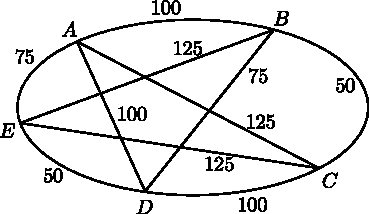
\includegraphics[scale=.8]{figures/ques-2.3.pdf}
		\caption{旅行商问题} \label{Fig:TSP-problem}
		\vspace{1cm}
				\begin{forest}
		  for tree={
		    draw,
		    circle,
		  },
		  [A
		  	[B, edge label={node[midway,left,font=\scriptsize]{100}}
		  		[C, edge label={node[midway,left,font=\scriptsize]{150}}
		  			[D, edge label={node[midway,left,font=\scriptsize]{100}}
		  				[E, edge label={node[midway,right,font=\scriptsize]{50}}
		  					[A, edge label={node[midway,right,font=\scriptsize]{75}}
		  					]]]
		  			[E, edge label={node[midway,right,font=\scriptsize]{125}}
		  				[D, edge label={node[midway,right,font=\scriptsize]{50}}
		  					[A, edge label={node[midway,right,font=\scriptsize]{100}}
		  					]]]
		  		][D, edge label={node[midway,right,font=\scriptsize]{75	}}
		  			[C, edge label={node[midway,left,font=\scriptsize]{100}}
		  				[E, edge label={node[midway,right,font=\scriptsize]{125}}
		  					[A, edge label={node[midway,right,font=\scriptsize]{75}}
		  					]]]
		  			[E, edge label={node[midway,right,font=\scriptsize]{50}}
		  				[C, edge label={node[midway,right,font=\scriptsize]{125}}
		  					[A, edge label={node[midway,right,font=\scriptsize]{125}}
		  					]]]
		  		][E, edge label={node[midway,right,font=\scriptsize]{125}}
					[C, edge label={node[midway,left,font=\scriptsize]{125}}
						[D, edge label={node[midway,right,font=\scriptsize]{100}}
							[A, edge label={node[midway,right,font=\scriptsize]{100}}
							]]]
					[D, edge label={node[midway,right,font=\scriptsize]{50}}
						[C, edge label={node[midway,right,font=\scriptsize]{100}}
							[A, edge label={node[midway,right,font=\scriptsize]{125}}
							]]]  		
		  		]
		  	][C][D][E]
		  ]
		\end{forest}
		\caption{旅行商问题状态空间图} \label{Fig:TSP-answer}
		\vspace{1cm}
		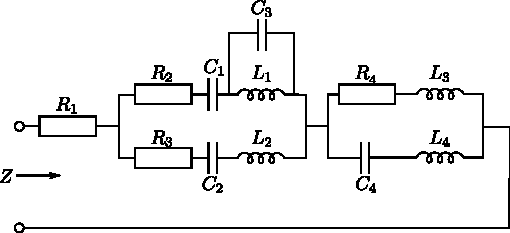
\includegraphics{figures/ques-2.4.pdf}
		\caption{电网络阻抗计算} \label{Fig:elec}
	\end{figure}
	
	\begin{figure}[H]
		\centering
		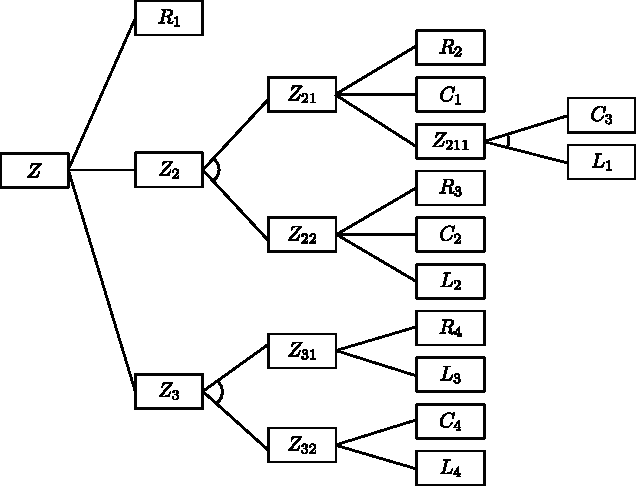
\includegraphics[scale=.8]{figures/ans-2.4.pdf}
		\caption{电网络阻抗计算与或解树} \label{Fig:and-or-tree-for-elec}
		\vspace{1cm}
		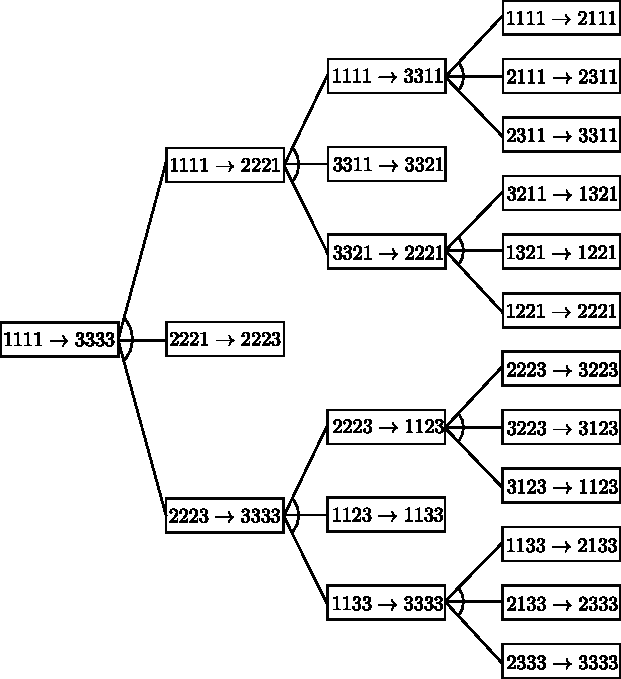
\includegraphics[scale=.8]{figures/ans-2.5.pdf}
		\caption{樊塔问题与或树} \label{Fig:and-or-tree-for-hannoi}
	\end{figure}

\begin{question}
把下列句子变换成子句形式:
	\begin{enumerate}
         \item $\left(\forall x\right) \left\{P\left(x\right) \to P\left(x\right)\right\}$
         \item $\forall x \forall y \left(\mathrm{On} \left(x,y\right) \to \mathrm{Above} \left(x,y\right) \right)$
         \item $\forall x \forall y \forall z \left(\mathrm{Above} \left(x,y\right) \wedge \mathrm{Above}\left(y,z\right) \to \mathrm{Above}\left(x,z\right) \right)$ 
         \item $\sim\left\{\left(\forall x\right)\left\{\left(\forall y)\left[p\left(y\right) \to p(f(x,y))\right] \wedge \left(\forall y \right) \left[Q(x,y) \to P(y) \right]\right\}\right\}\right\}$
	\end{enumerate}
\end{question}
\begin{solution}
	\begin{enumerate}
		\item $\sim P(x) \wedge P(x)$
		\item $\sim \mathrm{On}(x,y) \wedge \mathrm{Above}(x,y)$
		\item 
		\item 
	\end{enumerate}
\end{solution}

\begin{question}
用谓词演算公式表示下列英文句子(多用而不是省用不同谓词和项。例如不要用单一的谓词字母来表示每个句子)。
	\begin{quote}
		A computer system is intelligent if it can perform a task which, if performed by a human, requires intelligence. 
	\end{quote}
\end{question}
\begin{solution}
定义以下谓词:
	\begin{itemize}
		\item $\mathrm{INTLT}(x)$:	$x$ is intelligent.
		\item $\mathrm{PERFORM}(x,y)$:	$x$ can perform $y$.
		\item $\mathrm{REQUIRE}(x)$:		$x$ requires intelligence.
		\item $\mathrm{CMP}(x)$:		$x$ is a computer system.
		\item $\mathrm{HMN}(x)$:		$x$ is a human.
	\end{itemize} \par
则题中句子可以表达为
	\begin{multline*}
	\left( \exists t \right) \left( \exists y \right)
	\left[ \mathrm{HMN}(x) \vee \mathrm{PERFORM}(y,t) \vee \mathrm{REQUIRE}(t)
	\vee \mathrm{CMP}(x) \right. \\
	\left. \vee \mathrm{PERFORM}(x,t) \right] 
	\to \mathrm{INTLT}(x)
	\end{multline*}
\end{solution}

\begin{question}
把下列语句表示称语义网络描述:
	\begin{enumerate}
		\item All men are moral.
		\item Every cloud has a silver lining.
		\item All branch manager of DEC participate in a profit-sharing plan. 
	\end{enumerate}
\end{question}
\begin{solution}
如图\ref{Fig:semantic-net}。
	\begin{figure}[h]
		\centering
		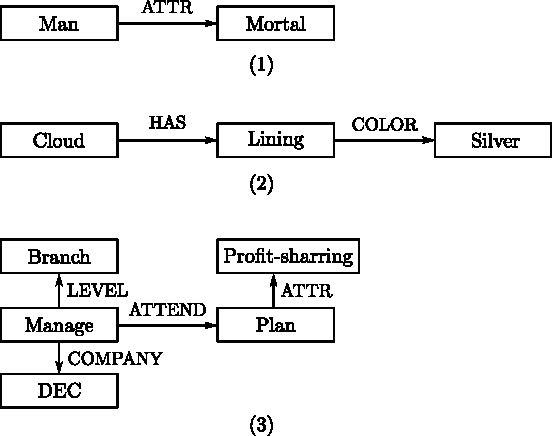
\includegraphics[scale=.9]{figures/ans-2.8.pdf}
		\caption{ 所求语义网络 } \label{Fig:semantic-net}
	\end{figure}
\end{solution}

\begin{question}
试构造一个描述你的寝室或办公室的框架系统。
\end{question}
\begin{solution}
以房间为例,如图\ref{Fig:semantic-my-room}。
	\begin{figure}[h]
		\centering
		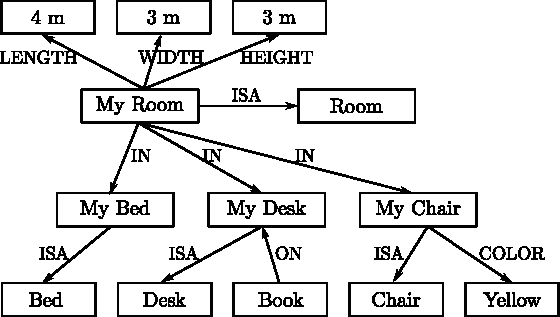
\includegraphics[scale=.9]{figures/ans-2.9.pdf}
		\caption{ 我的房间语义网络 } \label{Fig:semantic-my-room}
	\end{figure}
\end{solution}

\begin{question}
框架和本体有何关系与区别?
\end{question}
\begin{solution}
\end{solution}
\chapter{确定性推理}

\begin{question}
什么是图搜索过程?其中,重排OPEN表意味着什么?重排的原则是什么?
\end{question}	
\begin{solution}
图搜索的一般过程如下:
	\begin{enumerate}
		\item 建立一个只含有起始节点$S$的搜索图$G$,把$S$放到一个叫做OPEN的未扩展节点表中;
		\item 建立一个叫CLOSED的已扩展节点表,其初始为空表;
		\item LOOP:检查OPEN表是否为空,若为空,则失败退出;
		\item 选择OPEN表上的第一个节点,把它从OPEN表移出放进CLOSED表。并记该节点为节点$n$;
		\item 考察节点$n$是否为目标节点。若$n$为一目标节点,则有解并成功退出。此解是追踪图$G$中沿着指针从$n$到$S$这条路径而得到的(指针将在第7步中设置);
		\item 扩展节点$n$,生成一组子节点。把这些子节点中不是$n$的祖先的那些后继节点记入集合$M$。把$M$的这些成员作为$n$的后继节点添入图$G$中;
		\item 针对$M$中子节点的不同情况,分别作如下处理:
			\begin{itemize}
				\item 未曾在$G$中出现过的$M$成员设置一个通向其父节点(即节点$n$)的指针,并把$M$的这些成员加进OPEN表;(新生成的)
				\item 对已经在OPEN或CLOSED表上的每一个$M$成员,确定是否需要更改通到其父节点$n$的指针方向;(原生成但未扩展的)
				\item 对已在CLOSED表上的每个$M$成员,确定是否需要更改图$G$中通向它的每个后裔节点的指针方向;(原生成也扩展过的)
			\end{itemize}
		\item 按某一任意方式或按某个探试值,重排OPEN表;
		\item GO LOOP。
	\end{enumerate} \par
重排OPEN表意味着什么:在第(6)步中,将优先扩展哪个节点,不同的排序标准对应着不同的搜索策略。是否重新安排OPEN表,即是否按照某个试探值(或准则、启发信息等)重新对未扩展节点进行排序,将决定该图搜索过程是无信息搜索或启发式搜索。各种搜索策略的主要区别在于对OPEN表中节点的排列顺序不同。例如,广度优先搜索把先生成的子节点排在前面,而深度优先搜索则把后生成的子节点排在前面。\par
重排的原则当视具体需求而定,不同的原则对应着不同的搜索策略,如果想尽快地找到一个解,则应当将最有可能达到目标节点的那些节点排在OPEN表的前面部分,如果想找到代价最小的解,则应当按代价从小到大的顺序重排OPEN表。
\end{solution}

\begin{question}
试举例比较各种搜索方法的效率。
\end{question}	
\begin{solution}
几种搜索算法的效率:
	\begin{description}
		\item[宽度优先搜索] 只要问题有解,用宽度优先搜索总可以得到解,而且得到的是路径最短的解。宽度优先搜索盲目性较大,当目标节点距初始节点较远时将会产生许多无用节点,搜索效率低。
		\item[深度优先搜索] 搜索一旦进入某个分支,就将沿着该分支一直向下搜索。如果目标节点恰好在此分支上,则可较快地得到解。但是,如果目标节点不在此分支上,而该分支又是一个无穷分支,则就不可能得到解。所以深度优先搜索是不完备的,即使问题有解,它也不一定能求得解。所求得的解答路径不一定是最短路径。
		\item[有界深度优先搜索] 如果问题有解,且其路径长度$\leq dm$,则搜索过程一定能求得解。但是,若解的路径长度$> dm$,则搜索过程就得不到解。这说明在有界深度优先搜索中,深度界限的选择是很重要的。要恰当地给出$dm$的值是比较困难的。即使能求出解,它也不一定是最优解。
		\item[等代价搜索] 是宽度优先搜索的一种推广,不是沿着等长度路径断层进行扩展,而是沿着等代价路径断层进行扩展。搜索树中每条连接弧线上的有关代价,表示时间、距离等花费。若所有连接弧线具有相等代价,则简化为宽度优先搜索算法。
		\item[盲目搜索] 具有较大的盲目性,产生的无用节点较多,效率不高,耗费过多的计算空间与时间。
		\item[有序搜索] 利用启发信息,决定哪个是下一步要扩展的节点。选``最有希望''的节点作为下一个被扩展的节点。选择OPEN表上具有最小$f$值的节点作为下一个要扩展的节点, 又称为最佳优先搜索。正确选择估价函数对搜索结果具有决定性的作用。使用不能识别某些节点真实希望的估价函数会形成非最小代价路径;使用一个过多地估计了全部节点希望的估价函数又会扩展过多的节点。 
		\item[A算法] 虽提高了算法效率,但不能保证找到最优解。
		\item[A*算法] 搜索效率很大程度上取决于估价函数$h(n)$。一般来说,在满足$h(n)\leq h^*(n)$的前提下,$h(n)$的值越大越好。$h(n)$的值越大,说明它携带的启发性信息越多,A*算法搜索时扩展的节点就越少,搜索效率就越高。
	\end{description}

\end{solution}

\begin{question}
化为子句型有哪些步骤?请结合例子说明。
\end{question}	
\begin{solution}
任一谓词演算公式可以化成一个子句集。其变换过程由下列九个步骤组成:
	\begin{enumerate}
		\item 消去蕴涵符号,将蕴涵符号化为析取和否定符号;
		\item 减少否定符号的辖域,每个否定符号最多只用到一个谓词符号上,并反复应用狄·摩根定律;
		\item 对变量标准化,对哑元改名,以保证每个量词有其自己唯一的哑元;
		\item 消去存在量词,引入Skolem函数,消去存在量词。如果要消去的存在量词不在任何一个全称量词的辖域内,那么我们就用不含变量的Skolem函数即常量;
		\item 化为前束形,把所有全称量词移到公式的左边,并使每个量词的辖域包括这个量词后面公式的整个部分;
		\item 把母式化为合取范式, 反复应用分配律,将母式写成许多合取项的合取的形式,而每一个合取项是一些谓词公式和(或)谓词公式的否定的析取;
		\item 消去全称量词,消去前缀,即消去明显出现的全称量词;
		\item 消去连词符号(合取),用{合取项1, 合取项2}替换明显出现的合取符号;
		\item 更换变量名称,更换变量符号的名称,使一个变量符号不出现在一个以上的子句中。
	\end{enumerate}
\end{solution}

\begin{question}
如何通过消解反演求取问题的答案。
\end{question}	
\begin{solution}
给出一个公式集$S$和目标公式$L$,通过反证或反演来求证目标公式$L$,其证明步骤如下: 
	\begin{enumerate}
		\item 否定$L$,得$\sim L$; 
		\item 把$\sim L$添加到$S$中去; 
		\item 把新产生的集合$\left\{\sim L, S\right\}$化成子句集; 
		\item 应用消解原理,力图推导出一个表示矛盾的空子句。
	\end{enumerate}
\end{solution}

\begin{question}
什么叫合式公式?合式公式有哪些等价关系?
\end{question}	
\begin{solution}
合式公式的递归定义如下:
	\begin{enumerate}
		\item 原子谓词公式是合式公式。
		\item 若$A$为合式公式,则$\sim A$也是一个合式公式。
		\item 若$A$、$B$是合式公式,则$A \vee B$,$A \wedge B$、$A \to B$、$A \leftrightarrow B$也都是合式公式。
		\item 若$A$是合式公式,$x$为$A$中的自由变量,则$\left(\forall x\right) A$和$\left(\exists x\right) A$都是合式公式。
		\item 运用有限步上述规则(1)至(4)求得的那些公式是是合式公式。
	\end{enumerate}
等价关系有:
	\begin{enumerate}
		\item 否定之否定:$\sim(\sim P)=P$
		\item 蕴含与与或形式的等价:$\begin{cases}
		P\to Q = \sim P \vee Q\\
		\sim P\to Q = P \vee Q
		\end{cases}$ 
		\item 狄•摩根定律:$\begin{cases}
		\sim (P \vee Q) = \sim P \wedge \sim Q \\
		\sim (P \wedge Q) = \sim P \vee \sim Q 
		\end{cases}$
		\item 分配律:$\begin{cases}
		P \vee (Q \wedge R) = (P \vee Q) \wedge (P \vee R) \\
		P \wedge (Q \vee R) = (P \wedge Q) \vee (P \wedge R)
		\end{cases}$
		\item 交换律:$\begin{cases}
		P \vee Q = Q \vee P \\
		P \wedge Q = Q \wedge P
		\end{cases}$
		\item 结合律:$\begin{cases}
		P \vee (Q \vee R) = (P \vee Q) \vee R \\
		P \wedge (Q \wedge R) = (P \wedge Q) \wedge R
		\end{cases}$
		\item 逆否率:$(P \to Q) = (\sim Q \to \sim P)$
		\item 否定跨越量词:$\sim (\exists x) P(x) = (\forall x)[\sim P(x)]$
		\item 全称量词同与或连词:$\begin{cases}
		(\forall x)[P(x) \wedge Q(x)] = (\forall x) P(x) \wedge (\forall x) Q(x) \\
		(\forall x)[P(x) \vee Q(x)] = (\forall x) P(x) \vee (\forall x) Q(x)
		\end{cases}$
		\item 量词中的哑元:$\begin{cases}
		(\forall x) P(x) = (\forall y) P(y) \\
		(\exists x) P(x) = (\exists y) P(y)
		\end{cases}$
	\end{enumerate}
\end{solution}

\begin{question}
用宽度优先搜索求图\ref{Fig:maze}所示迷宫的出路。
	\begin{figure}[h]
		\centering
		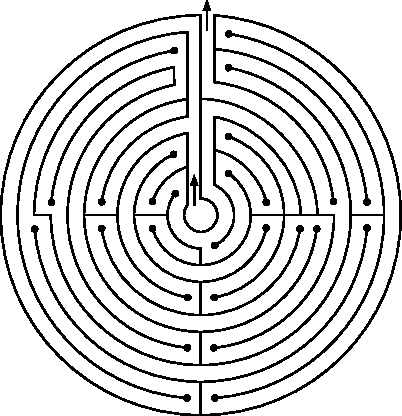
\includegraphics{figures/ques-3.6.pdf}
		\caption{迷宫一例} \label{Fig:maze}
	\end{figure}
\end{question}
\begin{solution}
在这个迷宫中,$S$是源节点,$F$是目标节点,$A$、$B$、$C$、$D$、$E$是$5$个具有二叉分支的节点,在每个节点处,都可能会出现两种路线,要么向左拐要么向右拐,我们在每个二叉节点处设立两个虚节点,以表示到该节点后的走向,向右拐为第一个虚节点,用下标$1$表示,向左拐为第二个虚节点,用下标$2$表示。例如,$A$节点处向右拐的虚节点用$A_1$表示,向左拐的虚节点用$A_2$表示。可以将该迷宫转换成一个有向图,如图\ref{Fig:maze-states-graph}。\par
	\begin{figure} [h]
		\centering
		\begin{tikzpicture}[->,>=stealth',shorten >=1pt,auto,node distance=1.3cm,
                    thick,main node/.style={circle,draw}]

  \node[main node] (S) {$S$};
  \node[main node] (A) [right of=S] {$A$};
  \node[main node] (A2) [above right of=A] {$A_2$};
  \node[main node] (A1) [below right of=A] {$A_1$};
  \node[main node] (B) [right of=A1] {$B$};
  \node[main node] (B2) [above right of=B] {$B_2$};
  \node[main node] (H) [above right of=B2] {$H$};
  \node[main node] (H2) [above right of=H] {$H_2$};
  \node[main node] (H1) [below right of=H] {$H_1$};
  \node[main node] (G) [above right of=H1] {$G$};
  \node[main node] (G1) [right of=G] {$G_1$};
  \node[main node] (G2) [above of=H2] {$G_2$};
  \node[main node] (B1) [below right of=B] {$B_1$};
  \node[main node] (C) [below right of=B1] {$C$};
  \node[main node] (C2) [above right of=C] {$C_2$};
  \node[main node] (C1) [below right of=C] {$C_1$};
  \node[main node] (D) [right of=C2] {$D$};
  \node[main node] (D2) [above right of=D] {$D_2$};
  \node[main node] (D1) [below right of=D] {$D_1$};
  \node[main node] (E) [right of=D2] {$E$};
  \node[main node] (E2) [above right of=E] {$E_2$};
  \node[main node] (E1) [below right of=E] {$E_1$};
  \node[main node] (F) [right of=C1] {$F$};
  

  \path[every node/.style={}]
  	(S) edge (A)
  	(A) edge (A1)
  		edge (A2)
  	(A1) edge (B)
  	(B) edge (B1)
  		edge (B2)
  	(B2) edge (H)
  	(H) edge (H1)
  		edge (H2)
  	(H2) edge (G)
  	(H1) edge (G)
  	(G) edge (G1)
  		edge [bend right] (G2)
  	(G2) edge [bend right] (H)
  	(B1) edge (C)
  	(C) edge (C1)
  		edge (C2)
  	(C2) edge (D)
  	(D) edge (D1)
  		edge (D2)
  	(D2) edge (E)
  	(E) edge (E1)
  		edge (E2)
  	(C1) edge (F);
\end{tikzpicture}
		\caption{迷宫状态空间图} \label{Fig:maze-states-graph}
	\end{figure}
除F节点是目标节点外,其余没有后继节点的虚节点都说明走入了死胡同。\par
利用深度优先搜索,其搜索树如图\subref*{Fig:maze-search-graph-dfs}所示,图中节点旁所标数字为节点扩展次序。所得到的解路径为:
\[ S \to A \to A_1 \to B \to B_1 \to C \to C_1 \to F \]
也就是说,从S出发,在A节点处不能左拐,而是直行,到B节点处右拐,到C节点也右拐,即可到达出口F。\par
利用宽度优先搜索,其搜索树如图\subref*{Fig:maze-search-graph-bfs}所示,图中节点旁所标数字为节点扩展次序。所得到的解路径为:
\[ S \to A \to A_1 \to B \to B_1 \to C \to C_1 \to F \]
由搜索过程可以看出,宽度优先搜索的效率低于深度优先搜索。
	\begin{figure} [h]
		\centering
		\captionsetup{justification=raggedright}
		\subfloat[深度优先搜索]{\label{Fig:maze-search-graph-dfs}\begin{tikzpicture}[->,>=stealth',shorten >=1pt,auto,node distance=1.3cm,
                    thick,main node/.style={circle,draw}]

  \node[main node] (S) {$S$};
  \node[main node] (A) [below of=S] {$A$};
  \node[main node] (A1) [below left of=A] {$A_1$};
  \node[main node] (A2) [below right of=A] {$A_2$};
  \node[main node] (B) [below of=A1] {$B$};
  \node[main node] (B1) [below left of=B] {$B_1$};
  \node[main node] (B2) [below right of=B] {$B_2$};
  \node[main node] (C) [below of=B1] {$C$};
  \node[main node] (C1) [below left of=C] {$C_1$};
  \node[main node] (C2) [below right of=C] {$C_2$};
  \node[main node] (F) [below of=C1] {$F$};
  

  \path[every node/.style={}]
  	(S) edge (A)
  	(A) edge (A1)
  		edge (A2)
  	(A1) edge (B)
  	(B) edge (B1)
  		edge (B2)
  	(B1) edge (C)
  	(C) edge (C1)
  		edge (C2)
  	(C1) edge (F);
\end{tikzpicture}}\qquad
		\subfloat[宽度优先搜索]{\label{Fig:maze-search-graph-bfs}\begin{tikzpicture}[->,>=stealth',shorten >=1pt,auto,node distance=1.3cm,
                    thick,main node/.style={circle,draw}]

  \node[main node] (S) {$S$};
  \node[main node] (A) [below of=S] {$A$};
  \node[main node] (A1) [below left of=A] {$A_1$};
  \node[main node] (A2) [below right of=A] {$A_2$};
  \node[main node] (B) [below of=A1] {$B$};
  \node[main node] (B1) [below left of=B] {$B_1$};
  \node[main node] (B2) [below right of=B] {$B_2$};
  \node[main node] (C) [below of=B1] {$C$};
  \node[main node] (C1) [below left of=C] {$C_1$};
  \node[main node] (C2) [below right of=C] {$C_2$};
  \node[main node] (F) [below of=C1] {$F$};
  \node[main node] (D) [below of=C2] {$D$};
  \node[main node] (B2) [below right of=B] {$B_2$};
  \node[main node] (H) [below right of=B2] {$H$};
  \node[main node] (H1) [below left of=H] {$H_1$};
  \node[main node] (H2) [below right of=H] {$H_2$};
  \node[main node] (G) [below of=H1] {$G$};
  \node[main node] (G') [below of=H2] {$G$};
  

  \path[every node/.style={}]
  	(S) edge (A)
  	(A) edge (A1)
  		edge (A2)
  	(A1) edge (B)
  	(B) edge (B1)
  		edge (B2)
  	(B2) edge (H)
  	(H) edge (H1)
  		edge (H2)
  	(H1) edge (G)
  	(H2) edge (G')
  	(B1) edge (C)
  	(C) edge (C1)
  		edge (C2)
  	(C1) edge (F)
  	(C2) edge (D);
\end{tikzpicture}}
	    \caption{迷宫搜索图}
	\end{figure}
\end{solution}

\begin{question}
用有界深度优先搜索方法求解图\ref{Fig:8-code}所示八数码难题。
	\begin{figure}[H]
		\centering
		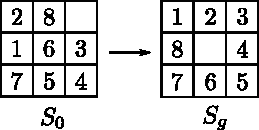
\includegraphics{figures/ques-3.7.pdf}
		\caption{八数码难题} \label{Fig:8-code}
	\end{figure}
\end{question}
\begin{solution}
定义操作符集:$F=\{f1,f2,f3,f4\}$,其中:$f1$表示空格右移;$f2$表示空格上移;$f3$表示空格左移;$f4$表示空格下移。\par
搜索时,节点的扩展顺序规定为按右、左、上、下方向移动空格。并设置深度界限为$8$。\par
	\begin{figure}[H]
		\centering
		\begin{tikzpicture}[->,>=stealth',shorten >=1pt, every node/.append style={on grid,node distance=1cm and 2cm},
                    every matrix/.append style={matrix of nodes,draw}]

\matrix (0) at(0,0) {2&8&\,\\ 1&6&3\\ 7&5&4\\};
\matrix [below left=of 0] (1) {2&\,&8\\ 1&6&3\\ 7&5&4\\};
\matrix [below right=of 0] (2) {2&8&3\\ 1&6&\,\\ 7&5&4\\};
\matrix [below left=of 2] (3) {2&8&3\\ 1&\,&6\\ 7&5&4\\};
\matrix [below right=of 2] (4) {2&8&3\\ 1&6&4\\ 7&5&\,\\};
\matrix [below right=of 4] (5) {2&8&3\\ 1&6&4\\ 7&\,&5\\};
\matrix [below left=of 5] (6) {2&8&3\\ 1&\,&4\\ 7&6&5\\};
\matrix [below right=of 5] (7) {2&8&3\\ 1&6&4\\ \,&7&5\\};
\matrix [below left=of 6] (8) {2&\,&3\\ 1&8&4\\ 7&6&5\\};
\matrix [below right=of 6] (9) {2&8&3\\ \,&1&4\\ 7&6&5\\};
\matrix [below left=of 8] (10) {2&3&\,\\ 1&8&4\\ 7&6&5\\};
\matrix [below right=of 8] (11) {\,&2&3\\ 1&8&4\\ 7&6&5\\};
\matrix [below left=of 11] (12) {1&2&3\\ \,&8&4\\ 7&6&5\\};
\matrix [below left=of 12] (13) {1&2&3\\ 8&\,&4\\ 7&6&5\\};
\matrix [below right=of 12] (14) {1&2&3\\ 7&8&4\\ \,&6&5\\};
\node [above=of 0] {$S_0$};
\node [left= 1cm of 13]{$S_g$};

\draw (0) edge node[above]{$f3$} (1) 
          edge node[above]{$f4$} (2);
\draw (2) edge node[above]{$f3$} (3)
          edge node[above]{$f4$} (4);
\draw (4) edge node[above]{$f3$} (5);
\draw (5) edge node[above]{$f2$} (6)
          edge node[above]{$f3$} (7);
\draw (6) edge node[above]{$f2$} (8)
          edge node[above]{$f3$} (9);
\draw (8) edge node[above]{$f1$} (10)
          edge node[above]{$f3$} (11);
\draw (11) edge node[above]{$f4$} (12);
\draw (12) edge node[above]{$f3$} (13)
           edge node[above]{$f4$} (14);

\end{tikzpicture}
		\caption{八数码难题} \label{Fig:8-digits-search-dfs}
	\end{figure}
由图\ref{Fig:8-digits-search-dfs}有界深度优先搜索树中可见,当$d=8$时,八数码难题的一个解为:
\[f4, f4, f3, f2, f2, f3, f4, f3 \, .\]
\end{solution}

\begin{question}
应用最新的方法表达传教士和野人问题,编写一个计算机程序,以求得安全渡过全部$6$个人的解答。(提示:在应用状态空间表示和搜索方法时,可用$(N_m,N_c)$来表示状态描述,其中$N_m$和$N_c$分别为传教士和野人的人数。初始状态为$(3,3)$,而可能的中间状态为$(0,1)$,$(0,2)$,$(0,3)$,$(1,1)$,$(2,1)$,$(2,2)$,$(3,0)$,$(3,1)$和$(3,2)$等。
\end{question}
\begin{solution}
略。
\end{solution}

\begin{question}
试比较宽度优先搜索、有界深度优先搜索及有序搜索的搜索效率,并以实例数据加以说明。
\end{question}
\begin{solution}
以八数码难题为例,下面比较宽度优先搜索、有界深度优先搜索及有序搜索的搜索效率。\par
	\begin{table}[htbp]
	\centering
	\begin{tabular}{p{50pt}p{40pt}p{40pt}p{140pt}}
		\toprule
		搜索方法 & CLOSE表长度 & OPEN表长度 & 搜索效率 \\
		\midrule
		宽度优先搜索 & 27 & 11 &
		优点:只要问题有解,总可以得到解,而且得到的是路径最短的解。\newline 缺点:盲目性较大,当目标节点距初始节点较远时将会产生许多无用节点,搜索效率低。 \\
		\midrule
		有界深度优先搜索 & 16 & 13 &
		如果问题有解,且其路径长度$\leq d_m$,则上述搜索过程一定能求得解。但是,若解的路径长度$>d_m$,则上述搜索过程就得不到解。这说明在有界深度优先搜索中,深度界限的选择是很重要的。要恰当地给出$d_m$的值是比较困难的。即使能求出解,它也不一定是最优解。\newline 搜索效率低。 \\
		\midrule
		有序搜索 & 5 & 7 &
		宽度优先搜索、深度优先搜索、等代价搜索均是有序搜索技术的特例。正确选择估价函数对搜索结果具有决定性的作用。\newline 搜索效率高。\\
		\bottomrule
	\end{tabular}
	\caption{搜索效率比较}\label{tab:comparison-of-searching}
	\end{table} 
\end{solution}

\begin{question}
一个机器人驾驶卡车,携带包裹(编号分别为\#1、\#2和\#3)分别投递到林(LIN)、吴(WU)和胡(HU) 3家住宅处。规定了某些简单的操作符,如表示驾驶方位的$\mathrm{drive}(x,y)$和表示卸下包裹的$\mathrm{unload}(z)$;对于每个操作符,都有一定的先决条件和结果。试说明状态空间问题求解系统如何能够应用谓词演算求得一个操作符序列,该序列能够生成一个满足$\mathrm{AT(\# 1,LIN) \wedge AT(\# 2,WU) \wedge AT(\# 3,HU)}$的目标状态。
\end{question}
\begin{solution}
初始状态可描述为:
	\begin{multline*}
	\mathrm{AT}(\#1, \sim \mathrm{LIN}) \wedge \mathrm{AT}(\#2, \sim \mathrm{WU}) \wedge \mathrm{AT}(\#3, \sim \mathrm{HU}) \wedge {} \\
	\mathrm{AT}(\#1, \mathrm{CAR}) \wedge \mathrm{AT}(\#2, \mathrm{CAR}) \wedge \mathrm{AT}(\#3, \mathrm{CAR})
	\end{multline*} 
目标状态可描述为:
	\begin{multline*}
	\mathrm{AT}(\#1, \mathrm{LIN}) \wedge \mathrm{AT}(\#2, \mathrm{WU}) \wedge \mathrm{AT}(\#3, \mathrm{HU}) \wedge {} \\
	\mathrm{AT}(\#1, \sim \mathrm{CAR}) \wedge \mathrm{AT}(\#2, \sim \mathrm{CAR}) \wedge \mathrm{AT}(\#3, \sim \mathrm{CAR})
	\end{multline*}
对每个操作符都有一定的先决条件和结果,如表\ref{tab:operators}:
	\begin{table}[htbp]
	\centering
	\begin{tabular}{p{50pt}p{130pt}p{130pt}}
		\toprule
		~ & 先决条件 & 结果 \\
		\midrule
		$\mathrm{drive}(x,y)$ & $\mathrm{AT}(\mathrm{CAR}, x)$ & $\mathrm{AT}(\mathrm{CAR}, y)$ \\
		\midrule
		$\mathrm{unload}(z)$ & $\mathrm{AT}(z, \mathrm{CAR}) \wedge \mathrm{AT}(\mathrm{CAR}, x)$ 
			& $\mathrm{AT}(z, \sim\mathrm{CAR}) \wedge \mathrm{AT}(x, x)$ \\
		\bottomrule
	\end{tabular}
	\caption{每个操作符的先决条件和结果}\label{tab:operators}
	\end{table} \par
至此,原问题就转换为:寻找一个可将初始状态转换到目标状态的操作序列,如何求得该操作序列。
\end{solution}

\begin{question}
规则演绎系统和产生式系统有哪几种推理方式?各自的特点为是什么?
\end{question}
\begin{solution}
规则演绎系统的推理方式有正向推理、逆向推理和双向推理。正向推理、逆向推理的特点见表\ref{tab:reasoning-of-rule-based-system};双向推理组合了正向推理和逆向推理的优点,克服了各自的缺点,具有更高的搜索求解效率。
	\begin{table}[htbp]
	\centering
	\begin{tabular}{p{80pt}p{110pt}p{110pt}}
		\toprule
		~ & 正向推理 & 逆向推理 \\
		\midrule
		推理方向 & 从if部分向then部分推理的过程,它是从事实或状况向目标或动作进行操作的 & 从then部分向if部分推理的过程,它是从目标或动作向事实或状况进行操作的 \\
		\midrule
		目标表达式 & 文字的析取 & 任意形式 \\
		\midrule
		事实表达式 & 任意形式 & 文字的合取 \\
		\bottomrule
	\end{tabular}
	\caption{规则演绎系统系统的推理方式}\label{tab:reasoning-of-rule-based-system}
	\end{table} 
	\par
产生式系统的推理方式有正向推理、逆向推理和双向推理。正向推理、逆向推理的特点见表\ref{tab:reasoning-of-production-system};双向推理结合了正向推理和逆向推理的长处,克服了两者的短处,其控制策略比两者都要复杂。
	\begin{table}[htbp]
	\centering
	\begin{tabular}{p{80pt}p{110pt}p{110pt}}
		\toprule
		~ & 正向推理 & 逆向推理 \\
		\midrule
		驱动方式 & 数据驱动 & 目标驱动 \\ 
		\midrule
		推理方法 & 从一组数据出发向前推到结论 & 从可能的解答出发,向后推理验证解答 \\ 
		\midrule
		启动方法 & 从一个事件启动 & 由询问关于目标状态的一个问题而启动 \\ 
		\midrule
		透明程度 & 不能解释其推理过程 & 可解释其推理过程 \\ 
		\midrule
		推理方向 & 由底向上推理 & 由顶向下推理 \\ 
		\midrule
		优点 & 算法简单、容易实现,允许用户一开始就把有关的事实数据存入数据库,在执行过程中系统能很快获得这些数据,而不必等到系统需要数据时才向用户询问 & 搜索目的性强,推理效率高 \\ 
		\midrule
		缺点 & 盲目搜索,可能会求解许多与总目标无关的子目标,每当总数据库内容更新后都要遍历整个规则库,推理效率较低 & 目标的选择具有盲目性,可能会求解许多假的目标;当可能的结论数目很多,即目标空间很大时,推理效率不高;当规则的右部是执行某种动作不是结论时,逆向推理不便使用 \\ 
		\midrule
		适用场合 & 主要用于已知初始数据,而无法提供推理目标,或解空间很大的一类问题,如监控、预测、规划、设计等问题的求解 & 主要用于结论单一或者已知目标结论,而要求验证的系统,如选择、分类、故障诊断等问题的求解 \\ 
		\midrule
		典型系统 & CLIPS,OPS & PROLOG \\
		\bottomrule
	\end{tabular}
	\caption{产生式系统的推理方式}\label{tab:reasoning-of-production-system}
	\end{table}
\end{solution}

\begin{question}
单调推理有何局限性?什么叫缺省推理?非单调推理系统如何证实一个节点的有效性?
\end{question}
\begin{solution}
单调系统不能很好地处理常常出现在现实问题领域中的3类情况,即不完全的信息、不断变化的情况、以及求解复杂问题过程中生成的假设。有两种方法可以证实节点的有效性:
	\begin{enumerate}
		\item 支持表。(SL (IN-节点表) (OUT-节点表)) \\
			如果某节点的IN节点表中提到的节点当前都是IN, 且OUT节点表中提到的节点当前都是OUT,则它是有效的。
		\item 条件证明。(CP(结论) (IN-假设) (OUT-假设)) \\
			条件证明(CP)的证实表示有前提的论点,无论何时,只要在IN假设中的节点为IN,OUT假设中的节点为OUT,则结论节点往往为IN,于是条件证明的证实有效。 
	\end{enumerate}
\end{solution}

\begin{question}
在什么情况下需要采用不确定推理或非单调推理?
\end{question}
\begin{solution}
不完全的信息、不断变化的情况、以及求解复杂问题过程中生成的假设。
\end{solution}

\begin{question}
下列语句是一些几何定理,把这些语句表示为基于规则的几何证明系统的产生式规则:
	\begin{enumerate}
		\item 两个全等三角形的各对应角相等。
		\item 两个全等三角形的各对应边相等。 
		\item 各对应边相等的三角形是全等三角形。
		\item 等腰三角形的两底角相等。 
	\end{enumerate}
\end{question}
\begin{solution}
产生式规则如下:
	\begin{enumerate}
		\item IF 两个三角形全等 THEN 各对应角相等;
		\item IF 两个三角形全等 THEN 各对应边相等;
		\item IF 两个三角形各对应边相等 THEN 两三角形全等;
		\item IF 它是等腰三角形 THEN 它的两底角相等。
	\end{enumerate}
\end{solution}

\end{document}